% faire une évolution des risques au cours du temps
% dosier bilan : toutes les soutenances, tout les doc, pas de doc temporaire
% doc papier cahier des charges signé, fiche de recette papier (+ version electronique)
% "Est ce que quelqu'un pourrait prendre la succession de notre projet"
% suite possible du projet ? compétence aquise ? -> à mettre dans la conclusion

\documentclass[xcolor=dvipsnames]{beamer}

\usepackage[utf8]{inputenc}
\usepackage[french]{babel}
\usepackage[T1]{fontenc}
%\usepackage{array}
%\usepackage{tabularx}
\usepackage{multirow}
%\usepackage{color}
%\usepackage{colortbl}
%\usepackage{textcomp}
\usepackage{xstring}
\usepackage{pgfbaseimage}

%%% MACRO %%%


% FIXME Prendre en compte les majuscule déjà présente
\makeatletter
\@ifpackageloaded{xstring}{
	\newcommand\smallcaps[1]{\StrLeft{#1}{1}\scriptsize\uppercase{\StrGobbleLeft{#1}{1}}\normalsize }
}{
	\newcommand\smallcaps[1]{\textsc{#1}}
}
\makeatother



%===============================================================================
% Définit un type de puce pour une liste. Si le pakage "pifont" est chargé, il 
% est utilisé, sinon on met un tiret.
\makeatletter
\@ifpackageloaded{pifont}{
	\newcommand\goodItemArrow[0]{\ding{226}}
}{
	\newcommand\goodItemArrow[0]{-}
}
\makeatother



%===============================================================================
% Item de liste avec spécification de la puce et paramètre écrit en gras.
\newcommand\functionality[1]{
	\item[\goodItemArrow] \textbf{#1}\\
}



%===============================================================================
% Commande \Euro indépendante des paquets chargés 
\makeatletter
\@ifpackageloaded{eurosym}{
	\newcommand\Euro[0]{\euro{}}
}{
	\@ifpackageloaded{textcomp}{
		\newcommand\Euro[0]{\texteuro}
	}{
		\newcommand\Euro[0]{Euro}
	}
}
\makeatother



%===============================================================================
% Accès à des variables dans le document. 
%\makeatletter
%\let\titleName\@title
%\let\subtitleName\@subtitle
%\let\authorName\@author
%\makeatother



% Titre de la section courante (que dans beamer)
%\secname 
% Titre de la sous-section courante (que dans beamer)
%\subsecname





\title[Final presentation]{Discrete 3D surfaces of revolution} % FIXME ou Discret revolution surfaces ?
\subtitle{Final presentation}
\author[Discret group]{Zied \smallcaps{Ben} \smallcaps{Othmane} \\
	Thomas \smallcaps{Benoist} \\
	Adrien \smallcaps{Bisutti} \\
	Lydie \smallcaps{Richaume}
} % FIXME Enlever les parenthèses
\institute{University of Poitiers}
\date{March 2\textsuperscript{nd}, 2016}

\usetheme{Madrid}
\usecolortheme{sidebartab}
\usefonttheme{professionalfonts}

\definecolor{fondtitre}{rgb}{0.0,0.35,0.7}
\setbeamercolor{palette primary}{bg=fondtitre}
\setbeamercolor{palette secondary}{bg=fondtitre!75!black}
\setbeamercolor{palette tertiary}{bg=fondtitre!55!black}
\setbeamercolor{palette quaternary}{bg=fondtitre!35!black}
\setbeamercolor{item}{fg=fondtitre}



%%% MACRO %%%

% Affichage du plan à chaque début de section
\AtBeginSection[]{
	\begin{frame}{Outline}
	  	\tableofcontents[currentsection, hideothersubsections]
	\end{frame}
}


% Nouvelle boîte pour le titre
\newenvironment<>{titleblock}[1]{%
	\setbeamercolor{block body}{fg=white, bg=fondtitre}%
	\begin{block}#2{#1}}{\end{block}}


% Vide la barre de navigation
\setbeamertemplate{navigation symbols}{}


% Todo
\newcommand{\todo}[1]{{\color{Red}TODO #1}}



%%% DOCUMENT %%%

\begin{document}

% intro avec contexte, objectif
% tavail (maquette, démo, liste outil)
% conduite projet (cout, paql, gantt, zoom gantt, risque (clients, rendue, serveur, évolution algo))
% conclusion (perspective, apport technique, livraison deux étapes)



%===============================================================================
%	TITRE
%===============================================================================

\begin{frame}
	\titlepage
	
\includegraphics[width=2cm]{../Images/logo-Xlim.png}
	\hfill
	
\includegraphics[width=2cm]{../Images/logo_univ_poitiers.png}
\end{frame}


%===============================================================================
%	PLAN
%===============================================================================

\begin{frame}{Outline}
	\tableofcontents[hidesubsection]
\end{frame}


%===============================================================================
%	INTRODUCTION
%===============================================================================
% intro avec contexte, objectif

\section{Introduction}


% --- Équipe -------------------------------------------------------------------
\subsection{Collaborators and clients}
	\begin{frame}{\subsecname}
		\begin{itemize}
			\item Clients:
				\begin{itemize}
					\item \'Eric \smallcaps{Andres} (Professor and former director of XLIM-SIC department)
					\item Gaëlle \smallcaps{Largeteau}-\smallcaps{Skapin} (University lecturer, Discrete geometry)
				\end{itemize}
			\item Exemple of final user:
				\begin{itemize}
					\item Aur\'elie \smallcaps{Mourier} (Artist)
				\end{itemize}
			\item Pedagogic Supervisor: 
				\begin{itemize}
					\item Philippe \smallcaps{Meseure} (Professor, Computer Graphics)
				\end{itemize}
		\end{itemize}
	\end{frame}


% --- Roles --------------------------------------------------------------------
\subsection{Roles}
	\begin{frame}{\subsecname}
		\begin{itemize}
			\item Team composition:
			\begin{itemize}
				\item Thomas \smallcaps{Benoist} - Project manager
				\item Zied \smallcaps{Ben} \smallcaps{Othmane} - Quality manager
				\item Adrien \smallcaps{Bisutti} - Risks manager
				\item Lydie \smallcaps{Richaume} - Tasks manager
			\end{itemize}
		\end{itemize}
	\end{frame}


% --- Contexte -----------------------------------------------------------------
\subsection{Context}
	\begin{frame}{\subsecname}
		\begin{itemize}
			\item \'Eric \smallcaps{Andres} and Ga\"elle \smallcaps{Largeteau}-\smallcaps{Skapin}
				developped a new algorithm to model discrete surfaces of revolution.
			\item Display the result with Mathematica
		\end{itemize}
		
		\begin{figure}
			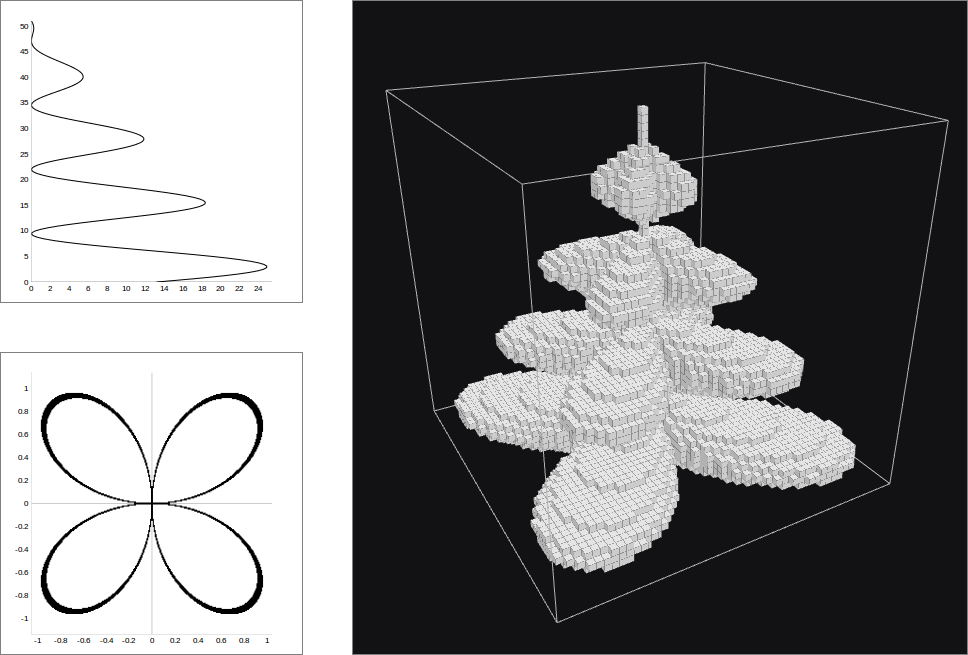
\includegraphics[height=4.7cm]{Images/context.png}
		\end{figure}
	
		\begin{itemize}
			\item Need of a tool useable by everyone and everywhere
		\end{itemize}
	\end{frame}
	

% --- Contexte -----------------------------------------------------------------
\subsection{Objectifs}
	\begin{frame}{Objectifs}
		\begin{itemize}
			\item Outil de visualisation de surfaces
				\begin{itemize}
					\item Visualiser en 3D, en coupe
					\item Choisir les méridianes et les courbes de révolution
			 		\item Exporter des objets obtenus
				\end{itemize}
		\end{itemize}
		\begin{itemize}
			\item Algorithme de construction des surfaces de révolution
				\begin{itemize}
					\item Fourni par les clients
					\item Possibilité d'évolution de l'algorithme
				\end{itemize}
		\end{itemize}
	\end{frame}



%===============================================================================
%	TRAVAIL RÉALISÉ
%===============================================================================

\section{Work achieved}
% tavail (maquette, démo, liste outil)


% --- Rappel et persective -----------------------------------------------------
\subsection{Maquette}
	\begin{frame}{\subsecname}
		\begin{itemize}
			\item Listes des fonctionnalitées
			\item Étude et transcription de l'algorithme
			\item Documentation technique
			\item Maquette
		\end{itemize}
		\begin{figure}
			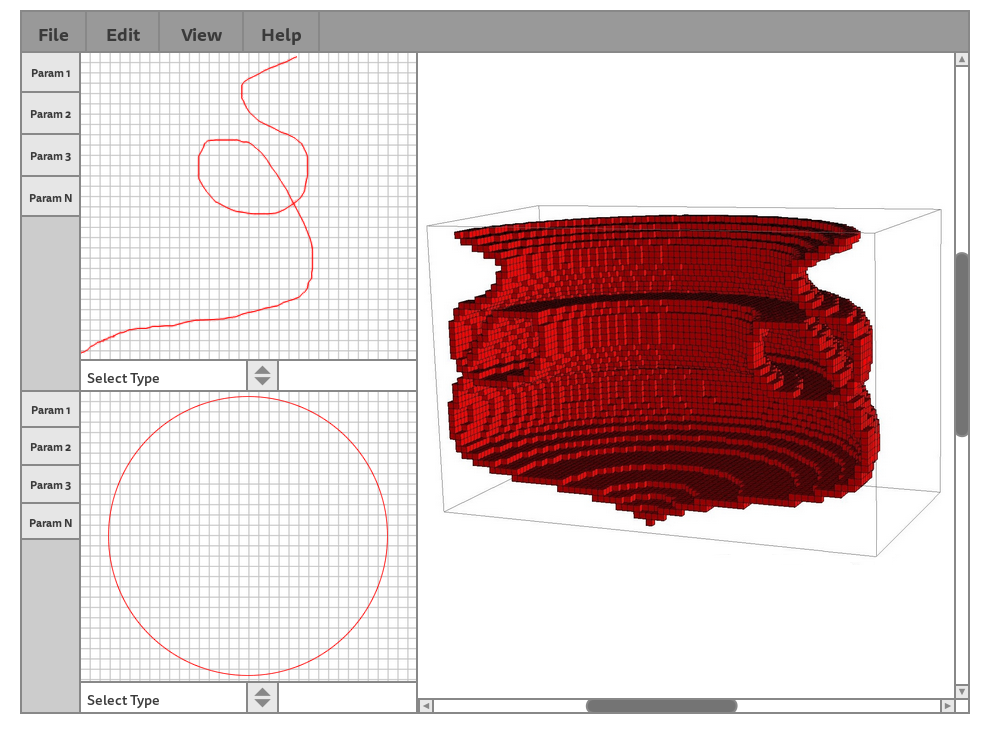
\includegraphics[height=5.7cm]{Images/maquette.png}
		\end{figure}
	\end{frame}


% --- Rappel et persective -----------------------------------------------------
\pgfdeclareimage[height=\paperheight, width=\paperwidth]{demo_bg}{Images/surface3d2.png}
\setbeamertemplate{background canvas}{\pgfuseimage{demo_bg}}
\subsection{Demonstration}
	\begin{frame}{\subsecname}
		\begin{center}
			\href
			{run:../../../ApplicationDiscret/Application/discreteSurface.html}
			{\subsecname}
		\end{center}
	\end{frame}

\setbeamertemplate{background canvas}[default]



%===============================================================================
%	CONDUITE DE PROJET
%===============================================================================
% conduite projet (cout, paql, gantt, zoom gantt, risque (clients, rendue, serveur, évolution algo))
\section{Gestion de projet}


% --- Gantt --------------------------------------------------------------------
\subsection{Gantt diagram}
	\begin{frame}{\subsecname}
		\begin{center}
			\href{run:}{Diagramme pr\'evisionnel}\\
			\bigskip
			\href{run:}{Diagramme r\'ealis\'e}
			% FIXME mettre les images
		\end{center}
	\end{frame}


	\begin{frame}{Zoom}
		\begin{center}
			\href{run:}{Diagramme pr\'evisionnel}\\
			\bigskip
			\href{run:}{Diagramme r\'ealis\'e}
			% FIXME mettre les images zoomer
		\end{center}
	\end{frame}


% --- Avancement ---------------------------------------------------------------
\subsection{Progress}
	\begin{frame}{\subsecname}
		\begin{figure}
			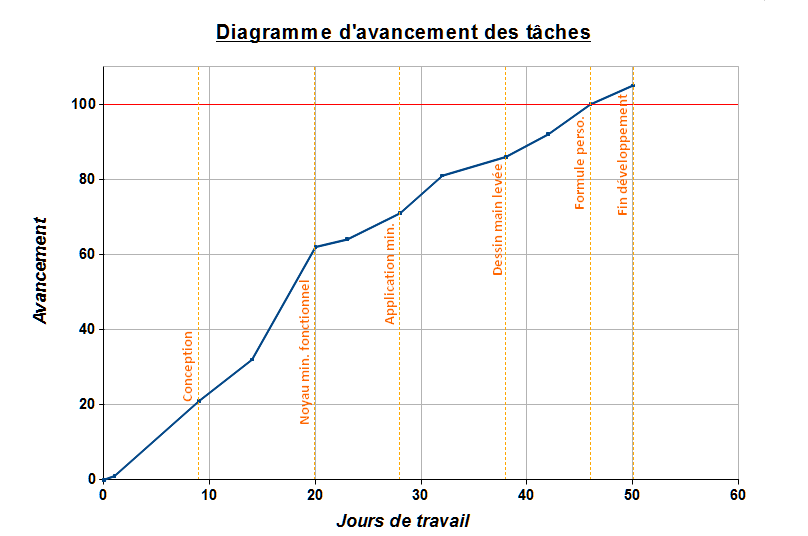
\includegraphics[width=12cm]{../Lancement/ImagesLancement/Avancement.png}
			% TODO régénéré
		\end{figure}
	\end{frame}


%--- risk ----------------------------------------------------------------------
\subsection{Risk evolution}


	% Tableau risque
	\newcommand{\legendeRisque}{
		\small
		\begin{tabular}{|c|c|c|c|}
			\hline
			Level & Gravity & Probability & Criticity \\
			\hline
			\hline
			% TODO traduire
			0 & Aucune & < 1\% & \multirow{2}*{No critical}\\
			\cline{1-3}
			1 & Faible (marges) & de 1\% à 5\% & \\
			\hline
			2 & Significative & de 5\% à 20 \% & \multirow{2}*{Critical}\\
			\cline{1-3}
			3 & Danger & > 20\% & \\
			\hline
		\end{tabular}
	}



% TODO vérifier si c'est les bon
% --- Risque -------------------------------------------------------------------
	\begin{frame}{\subsecname}
		\begin{itemize}
			\item Server linked problems
		\end{itemize}
		\begin{figure}
			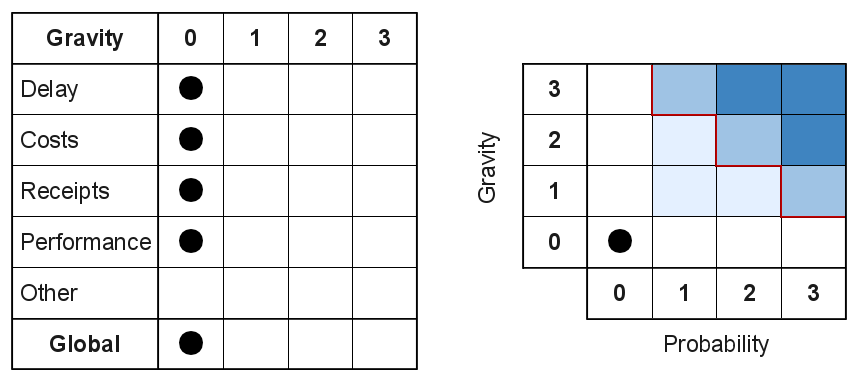
\includegraphics[width=8cm]{Images/risque_serveur.png}
		\end{figure}
		\begin{center}
			\legendeRisque
		\end{center}
	\end{frame}


% --- Risque -------------------------------------------------------------------
	\begin{frame}{\subsecname}
		\begin{itemize}
			\item New clients {\color{white}p} % fix la position par raport à la diapo suivante/précédentes
		\end{itemize}
		\begin{figure}
			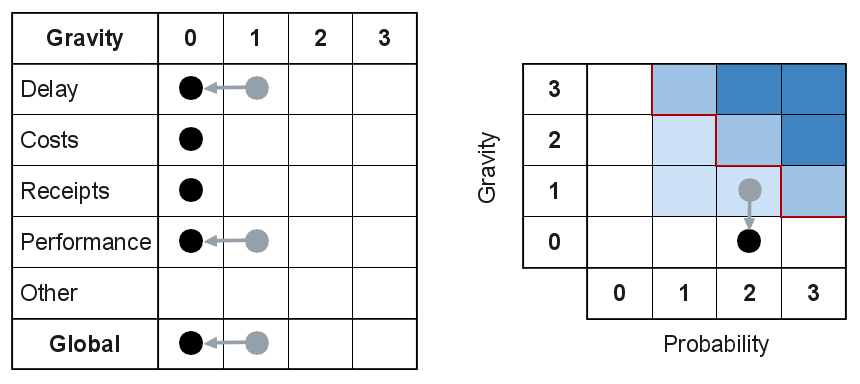
\includegraphics[width=8cm]{Images/risque_nouveau_client.png}
		\end{figure}
		\begin{center}
			\legendeRisque
		\end{center}
	\end{frame}
	
	
% --- Risque -------------------------------------------------------------------
	\begin{frame}{\subsecname}
		\begin{itemize}
			\item Generation algorithm evolution
		\end{itemize}
		\begin{figure}
			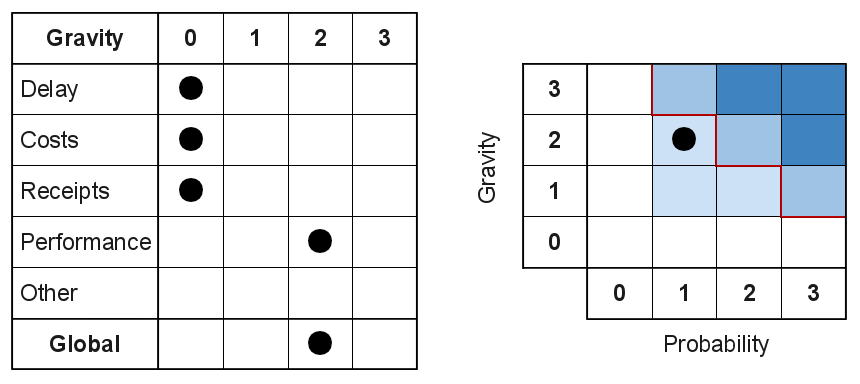
\includegraphics[width=8cm]{Images/risque_performance.png}
		\end{figure}
		\begin{center}
			\legendeRisque
		\end{center}
	\end{frame}	
	
	
% --- Risque -------------------------------------------------------------------
	\begin{frame}{\subsecname}
		\begin{itemize}
			\item Risque de rendu
		\end{itemize}
		\begin{figure}
			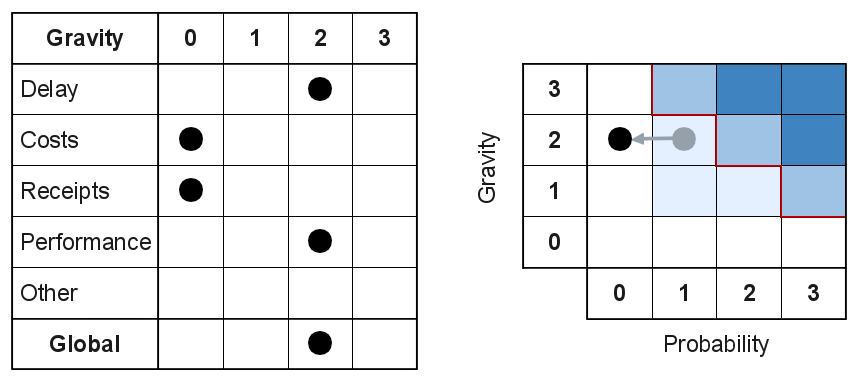
\includegraphics[width=8cm]{Images/risque_rendu.png}
		\end{figure}
		\begin{center}
			\legendeRisque
		\end{center}
	\end{frame}


% --- PAQL ---------------------------------------------------------------------
\subsection{Quality insurance plan}
	\begin{frame}{\subsecname}
		\begin{columns}
			\begin{column}{8cm}
				\begin{figure}
					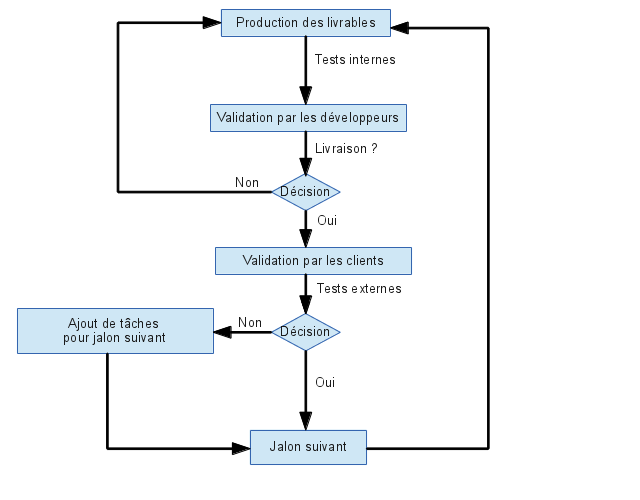
\includegraphics[width=8cm]{../Suivi/PAQL.png}
				\end{figure}
			\end{column}
			\begin{column}{4cm}
				Validation par les clients à chaque jalon.
			\end{column}
		\end{columns}
	\end{frame}


% --- Coût ---------------------------------------------------------------------
\subsection{Costs}
	\begin{frame}{\subsecname}
		\begin{figure}
			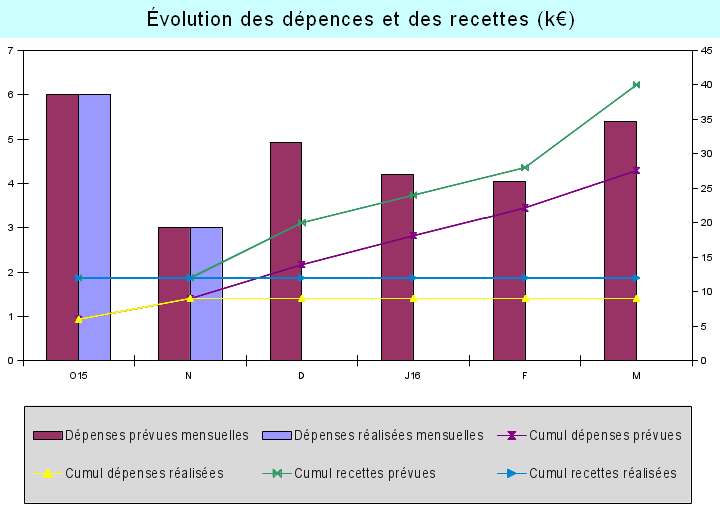
\includegraphics[height=7.5cm]{../Suivi/Cout.png}
			% FIXME généré l'image qui va bien
		\end{figure}
	\end{frame}



%===============================================================================
%	CONCLUSION
%===============================================================================
% conclusion (perspective, apport technique, livraison deux étapes)
\section{Conclusion}


% --- Rappel et persective -----------------------------------------------------
\begin{frame}{\secname}
	\begin{itemize}
		\item Apport technique javascript (classe, worker, blob, webgl, etc.)
		\item Livraison en deux étapes
		\item Perspectives
	\end{itemize}
\end{frame}


% --- Remerciment --------------------------------------------------------------
\begin{frame}{}
	\bigskip
	\bigskip
	\begin{titleblock}{}
		\begin{center}
			\smallskip
			\Large Discrete 3D surfaces of revolution\\
			\medskip
			\small Final presentation
			\smallskip
		\end{center}
	\end{titleblock}

	\bigskip
	\begin{center}
		Thanks for your attention.\\
		\medskip
		Are there any questions\,?			
	\end{center}

	\bigskip
	\bigskip
	
\includegraphics[width=2cm]{../Images/logo-Xlim.png}
	\hfill
	
\includegraphics[width=2cm]{../Images/logo_univ_poitiers.png}
\end{frame}



\end{document}
